%%%%%%%%%%%%%%
\section{Thursday 13 September:  Triangle Mesh}
%%%%%%%%%%%%%

HW \#2 Triangle Mesh

Move around based on user clicks.  

\

Primitive called OpenGL Triangle Strip

\

\begin{tikzpicture}[x=50mm, y=50mm]
	\coordinate (v0) at (0,0);
	\coordinate (v1) at (1,0);
	\coordinate (v2) at (2,0);
	\coordinate (v3) at (3,0);
	\coordinate (v4) at (0,1);
	\coordinate (v5) at (1,1);
	\coordinate (v6) at (2,1);
	\coordinate (v7) at (3,1);
	\path (v0) node [below] {$v_0$};
	\path (v1) node [below] {$v_1$};
	\path (v2) node [below] {$v_2$};
	\path (v3) node [below] {$v_3$};
	\path (v4) node [above] {$v_4$};
	\path (v5) node [above] {$v_5$};
	\path (v6) node [above] {$v_6$};
	\path (v7) node [above] {$v_7$};
	\draw [ultra thick] (v0) -- (v4) -- (v1) -- (v5) -- (v2) -- (v6) -- (v3) -- (v7);
	\draw [-triangle 60] (v0) -- ($0.5*(v0)+0.5*(v4)$);
	\draw [-triangle 60] (v4) -- ($0.5*(v4)+0.5*(v1)$);
	\draw [-triangle 60] (v1) -- ($0.5*(v1)+0.5*(v5)$);
	\draw [-triangle 60] (v5) -- ($0.5*(v5)+0.5*(v2)$);
	\draw [-triangle 60] (v2) -- ($0.5*(v2)+0.5*(v6)$);
	\draw [-triangle 60] (v6) -- ($0.5*(v6)+0.5*(v3)$);
	\draw [-triangle 60] (v3) -- ($0.5*(v3)+0.5*(v7)$);
	\draw [dashed, red] (v0) -- (v3);
	\draw [dashed, red] (v4) -- (v7);
	\coordinate (C) at (${sqrt(2)/(2+sqrt(2))}*(v0)+{1/(2+sqrt(2))}*(v1)+{1/(2+sqrt(2))}*(v4)$);
	\draw [-triangle 60] ($(C)+({0.2*cos(240)},{0.2*sin(240)})$) arc (240:0:0.2);
	\path (C) node [below right, align=center] {Winding \\ order};
	\coordinate (D) at (${sqrt(2)/(2+sqrt(2))}*(v5)+{1/(2+sqrt(2))}*(v1)+{1/(2+sqrt(2))}*(v4)$);
	\draw [triangle 60-] ($(D)+({0.2*cos(60)},{0.2*sin(60)})$) arc (60:-210:0.2);
\end{tikzpicture}

\

{\it Vertex List} \quad Array with vertices or vertex array.

$\{ \{ x_0, y_0, z_0 \}, \{ x_1, y_1, z_1\}, \dots, \{x_7, y_7, z_7\}\}$

\

{\it Index List} \quad Order in which the vertices form triangles.

First three vertices define first triangle, next vertex creates another triangle.  

$\{0,4,1,5,2,6,3,7\}$

\

Vertex list gives {\it geometry}, index list gives {\it topology} -- connectivity with neighbors.

\begin{tikzpicture}[x=9mm, y=10mm]
	\clip (-7,-4.1) rectangle (13,4.1);
	\coordinate (A) at (-5,2);
	\coordinate (B) at (-5,-2);
	\coordinate (C) at (5,2);
	\coordinate (D) at (5,-2);
	\coordinate (E) at (-5,0);
	\coordinate (F) at (5,0);
	\coordinate (G) at (5,4);
	\coordinate (H) at (5,-4);
	\coordinate (I) at (10,0);
	\draw (E) ellipse (1 and 2);
	\draw (F) ellipse (1 and 2);
	\draw [name path=ellipse] (F) ellipse (2 and 4);
	\path [name path=oline] (I) -- ({10-1.1*sqrt(21)},{1.1*4});
	\path [name intersections={of = ellipse and oline}];
	\coordinate (J) at (intersection-1);
	\coordinate (K) at (intersection-2);
	\path [name path=nline] (I) -- ({10-1.1*sqrt(21)},-{1.1*4});
	\path [name intersections={of = ellipse and nline}];
	\coordinate (L) at (intersection-1);
	\coordinate (M) at (intersection-2);
	\fill [white] (C) rectangle ($(C)+(-3,-4)$);
	\draw (A) -- (C);
	\draw (B) -- (D);
	\draw (J) -- (I) -- (L);
	\draw [dashed, triangle 60-triangle 60] (-5,3) -- (-5,0) -- (12,0);
	\path (-5,3) node [above] {$y$};
	\path (12,0) node [right] {$x$};
\end{tikzpicture}

\

\begin{tikzpicture}[x=9mm, y=10mm]
	\clip (-7,-4.1) rectangle (13,4.1);
	\draw [-triangle 60, dashed] (-5,0) -- (12,0);
	\draw [-triangle 60, dashed] (-5,0) -- (-5,2);
	\draw (-6,0) circle (0pt);
	\coordinate (A) at (-5,0);
	\coordinate (B) at (-5,-2);
	\coordinate (C) at (5,-2);
	\coordinate (D) at (5,-4);
	\coordinate (E) at (10,0);
	\draw (A) -- (B) -- (C) -- (D) -- (E);
	\path (A) node [left] {${(x_0,y_0)}$};
	\path (B) node [below left] {$(x_1,y_1)$};
	\path (C) node [below left] {$(x_2,y_2)$};
	\path (D) node [below] {$(x_3,y_3)$};
	\path (E) node [below right] {$(x_4,y_4)$};
	\path (-5,3) node [above] {$y$};
	\path (12,0) node [right] {$x$};
\end{tikzpicture}

\

Rotate about $x$-axis.  

\

\begin{tikzpicture}[x=7mm, y=7mm]
	\draw [-triangle 60] (0,0) -- (0,5) node [above] {$y$};
	\draw [-triangle 60] (0,0) -- (-5,0) node [left] {$z$};
	\draw (0,0) circle (4);
	\draw [dashed] circle (2);
	\fill (0,-2) circle (2pt);
	\fill (0,-4) circle (2pt);
	\path (0,-2) node [below right] {$(x_1,y_1)$};
	\path (0,-2) node [below left] {$(x_2,y_2)$};
	\path (0,-4) node [below] {$(x_3,y_3)$};
	\path (0,6) node {Front (tip) View};
\end{tikzpicture}
\hfill
\begin{tikzpicture}[x=7mm, y=7mm]
	\draw [-triangle 60] (0,0) -- (0,5) node [above] {$y$};
	\draw [-triangle 60] (0,0) -- (-5,0) node [left] {$z$};
	\draw (0,0) circle (4);
	\coordinate (A) at (0,0);
	\coordinate (B) at ({4*cos(330)},{4*sin(330)});
	\coordinate (C) at (0,{4*sin(330)});
	\draw (A) -- (B) -- (C) -- (A);
	\fill (0,-4) circle (2pt) node [below] {$(x_{i0},y_{i0}, 0)$};
	\fill (B) circle (2pt) node [below right] {$(x_{i0}, y_{i0} \cos \theta, y_{i0} \sin \theta)$};
	\draw (C) rectangle ($(C)+(0.3,0.3)$);
	\path (B) -- (C) node [ midway, below] {$y_{i0} \sin \theta$};
	\path (A) -- (C) node [ midway, left] {$y_{i0} \cos \theta$};
	\path (A) -- (B) node [ midway, above] {$y_{i0}$};
	\path ({1*cos(300)},{1*sin(300)})  node {$\theta$};
\end{tikzpicture}


\

Positive rotation is counter-clockwise when the axis is pointing towards you.  

\

Let $np$ be the number of points to be rotated, and $nm$ be the number of steps of the rotation.

\

Vertex list:  

\qquad $(x_{ij}, y_{ij}, z_{ij}) = (x_{i0}, \cos \theta y_{i0}, \sin\theta y_{i0})$ with $\displaystyle\theta = \frac{2\pi}{nm} j$ for $0 \le i \le np$ and  $0 \le j \le nm$.


\

\subsection{Array of a Rotated Surface}

The bottom and top rows are the same.  

Vertical lines represent different $x$ values

Horizontal lines represent different values of $\theta$.  

\

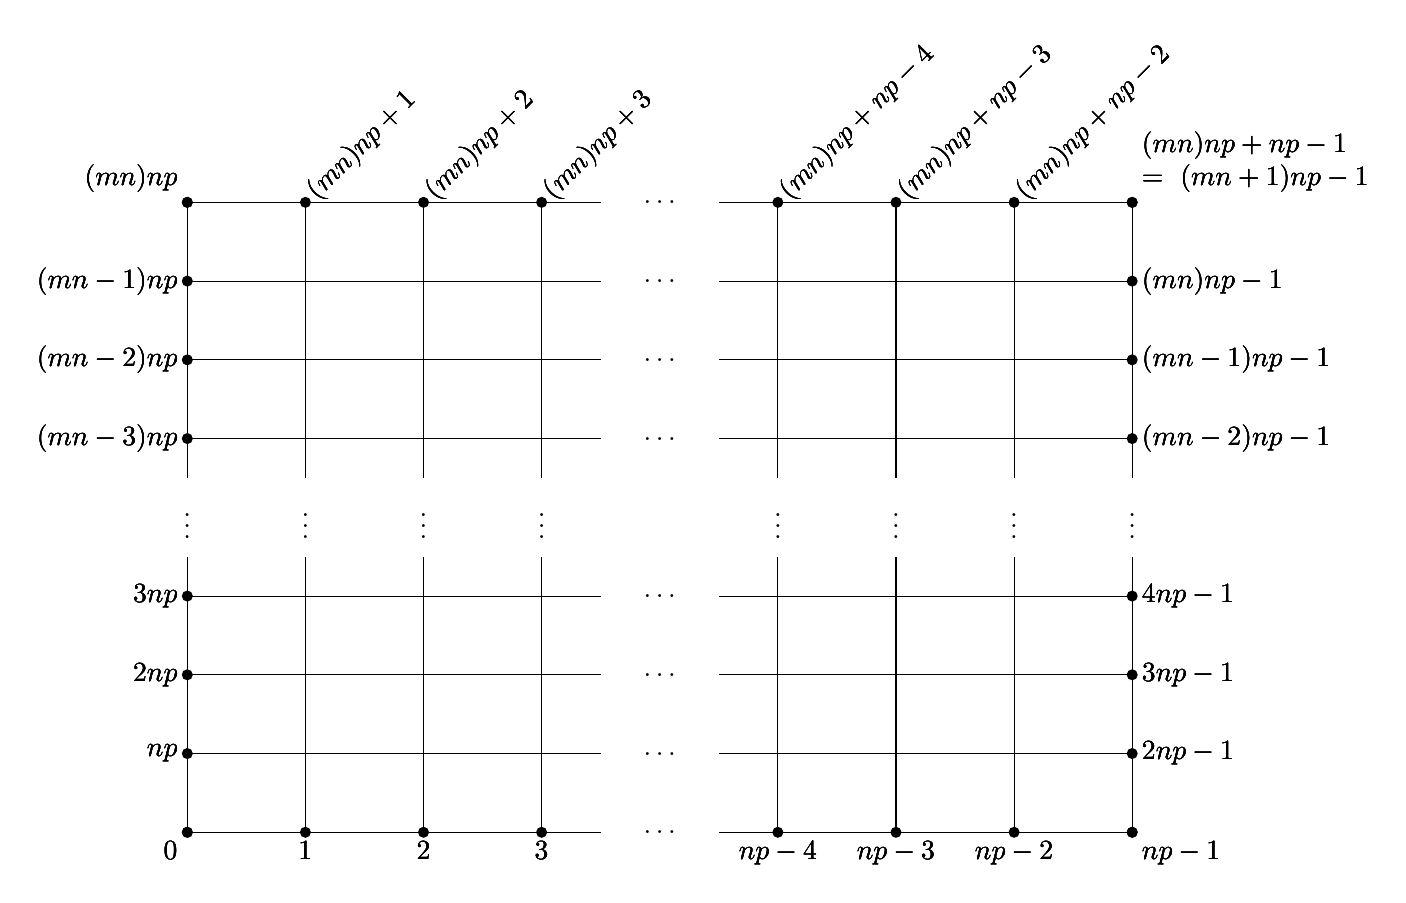
\begin{tikzpicture}[x=15mm,y=10mm]
	\foreach \i in {0,1,2,3}{
		% Lower left
		\draw (0,\i) -- (3.5, \i);
		\draw (\i,0) -- (\i,3.5);
		\path (\i,4) node {$\vdots$};
		\path (4,\i) node {$\dots$};
		\fill (0,\i) circle (2pt);
		\fill (\i,0) circle (2pt);
		% Upper left
		\draw (\i,4.5) -- (\i,8);
		\draw (0,{\i+5}) -- (3.5,{\i+5}); 
		\path (4,{\i+5}) node {$\dots$};
		\fill (0,{\i+5}) circle (2pt);
		\fill (\i,8) circle (2pt);
		% Lower right
		\draw ({\i+5},0) -- ({\i+5},3.5);
		\draw (4.5,{\i}) -- (8,{\i}); 
		\path ({\i+5},4) node {$\vdots$};
		\fill ({\i+5},0) circle (2pt);
		\fill (8, {\i}) circle (2pt);
		% Upper right
		\draw ({\i+5},4.5) -- ({\i+5},8);
		\draw (4.5,{\i+5}) -- (8,{\i+5}); 
		\fill ({\i+5},8) circle (2pt);
		\fill (8,{\i+5}) circle (2pt);
		\path (0,0) node [below left] {$0$};
		\path (1,0) node [below] {$1$};
		\path (2,0) node [below] {$2$};
		\path (3,0) node [below] {$3$};
		\path (5,0) node [below] {$np-4$};
		\path (6,0) node [below] {$np-3$};
		\path (7,0) node [below] {$np-2$};
		\path (8,0) node [below right] {$np-1$};
		\path (0,1) node [left] {$np$};
		\path (0,2) node [left] {$2np$};
		\path (0,3) node [left] {$3np$};
		\path (0,5) node [left] {$(mn-3)np$};
		\path (0,6) node [left] {$(mn-2)np$};
		\path (0,7) node [left] {$(mn-1)np$};
		\path (0,8) node [above left] {$(mn)np$};
		\path (8,1) node [right] {$2np-1$};
		\path (8,2) node [right] {$3np-1$};
		\path (8,3) node [right] {$4np-1$};
		\path (8,5) node [right] {$(mn-2)np - 1$};
		\path (8,6) node [right] {$(mn-1)np - 1$};
		\path (8,7) node [right] {$(mn)np - 1$};
		\path (8,8) node [above right, align=left] {$(mn)np + np - 1$ \\ $= \ (mn+1)np - 1$};
		\path (1,8) node [rotate=45, right] {$(mn)np + 1$};
		\path (2,8) node [rotate=45, right] {$(mn)np + 2$};
		\path (3,8) node [rotate=45, right] {$(mn)np + 3$};
		\path (5,8) node [rotate=45, right] {$(mn)np + np-4$};
		\path (6,8) node [rotate=45, right] {$(mn)np + np-3$};
		\path (7,8) node [rotate=45, right] {$(mn)np + np-2$};
%		\path (,8) node [above, rotate=45] {$$};
%		\path (0,) node [left] {$$};
	}
	
\end{tikzpicture}

How many vertices?  $np\times (nm+1)$

How many cells? $(np-1)(nm)$

How many triangles? $2(np-1)(nm)$

\

Vertex List 

{\tt loop over theta}

\qquad {\tt loop over x}

\

{\tt for theta in range (mn+1):}

\qquad {\tt for x in range (np):}

\qquad \qquad {\tt x(x,theta), y(x,theta), z(x,theta)}

\

{\color{red}  I have this in my notes, but I think it's wrong. 

$\{ 
	x_{0,0}, y_{0,0}, z_{0,0},
	x_{0,1}, y_{0,1}, z_{0,1},
$
}

\

$\{ 
	x_{0,0}, y_{0,0}, z_{0,0},
	x_{1,0}, y_{1,0}, z_{1,0},
	\dots,
	x_{np-1,0}, y_{np-1,0}, z_{np-1,0},
$

\qquad$
	x_{0,1}, y_{0,1}, z_{0,1},
	\dots,
$

\qquad \qquad $
	\dots, x_{np-1,mn}, y_{np-1,mn}, z_{np-1,mn},
\}$

\

Index List, using {\it primitive restart index}

$\{ 0, np, 1, np+1, 2, np+2, \dots, np-1, 2np-1, $ restart,

$np, 2np, np+1, 2np+1, \dots, 2np-2, 3np-2, 2np-2, 3np-1,$ restart,

$\vdots$

$(mn-1)np, (mn)np, (mn-1)np + 1, (mn)np+1, \dots, (mn)np-1, (mn+1)np - 1$, restart $\}$







